\section{三}

\subsection{三藏}
《增一阿含經‧序品》中則加雜藏為四藏,《分別功德論》及《成實論》又將雜藏分為雜藏及菩薩藏,成了五藏。
\begin{itemize}
  \item 經 \item 律 \item 論
\end{itemize}


\subsection{三法印}
即是用三句話來印證諸法,合乎這三句話的標準,便印可它是合於佛法的正見,否則便是魔外偏妄的邪見
\begin{itemize}
  \item 諸行無常
  \item 諸法無我
  \item 涅槃寂靜
\end{itemize}

\subsection{三無漏學}
由持戒清淨之後,修禪才能得正定;由正定的定力,可以產生無漏的慧力;再由慧力來指導持戒。
唯有藉著空慧或無漏慧的正見,持戒才會恰如其分,修禪才不致歧入魔境。
\begin{itemize}
  \item 戒
  \item 定
  \item 慧
\end{itemize}

\subsection{三毒、三不善根、三火}
\begin{itemize}
  \item 贪
  \item 嗔
  \item 痴
\end{itemize}



\subsection{三世}
\begin{itemize}
  \item 过去世
  \item 现在世
  \item 未来世
\end{itemize}

\subsection{三轉四諦}
\begin{itemize}
  \item 示轉:說明此是苦、此是集、此是滅、此是道。
  \item 勸轉:說明苦應知、集應斷、滅應證、道應修。
  \item 證轉:說明苦者我已知、集者我已斷、滅者我已證、道者我已修。
\end{itemize}

\subsection{三苦}
\begin{itemize}
  \item 苦苦
  \item 壞苦
  \item 行苦
\end{itemize}

\subsection{三連鎖}
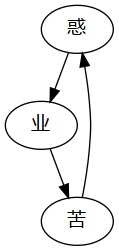
\includegraphics[scale=0.5]{释家/images/三连锁.png}
\begin{itemize}
  \item 惑:過去世的無明,現在世的愛及取。
  \item 業:過去世的行,現在世的有。
  \item 苦:現在世的識、名色、六入、觸、受,未來世的生及老死。
\end{itemize}

\subsection{三諦偈}
\begin{quote}
  眾因緣生法,我說即是無,亦為是假名,亦是中道義。
\end{quote}
緣起無自性,所以是空;為了引導眾生,又不得不說種種的法,這些法既無自性,所以是假名而說。假名之法,即是世俗諦。

\subsection{三求}
\begin{itemize}
  \item 欲求  \item 有求  \item 梵行求
\end{itemize}

\subsection{三身}
\begin{itemize}
  \item 法身是諸佛的本體
  \item 報身是諸佛的個體
  \item 化身則為適應眾生的要求而做廣大的救濟。
\end{itemize}


\subsection{三相}
\begin{enumerate}
  \item 遍計所執相─此即是錯覺或幻覺。
  \item 依他起相─此即是說因緣所生之法,其中含有從常識世界到科學世界的現象,一切均係依他之緣而生起之相狀。
  \item 圓成實相─此即是諸法平等的真如實相。
\end{enumerate}
\subsection{三自性}
\begin{enumerate}
  \item 遍計執性─妄分別性
  \item 依他起性─緣起性
  \item 圓成實性─真實性
\end{enumerate}
\subsection{三無性}
即是:將以上的三相,歸著於根本,都不離心。
\begin{enumerate}
  \item 遍計所執相是心的表象,沒有特別的自性存在,此稱為相無自性。
  \item 依他起相是因緣生法,因緣的總管也是心,故亦沒有特殊的自性,此稱為生無自性。
  \item 圓成實相是清淨心所緣,同樣是離心即無其自性,此稱為勝義無自性。
\end{enumerate}
\subsection{三時了未了說}
這是對於思想判釋的方法。《解深密经》認為,佛陀始對小乘人說四諦法,是未了義(不究竟)說;次對菩薩說諸法無自性,不生亦不滅,也是未了義說;本經說三相三無性,始為了義之說。本經對三乘佛法以了義未了義來判釋的方法,給予後世教判思想的影響很大。
